\documentclass{article}
\usepackage{tikz}
\usetikzlibrary{arrows.meta}

\begin{document}

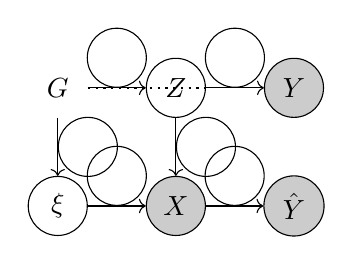
\begin{tikzpicture}[node distance=1.5cm, auto]
    \tikzstyle{every node}=[circle, draw, minimum size=0.75cm]

    % Nodes
    \node (G) [draw=none] {$G$};
    \node (Z) [right of=G] {$Z$};
    \node (Y) [right of=Z, fill=gray!40] {$Y$};
    \node (X) [below of=Z, fill=gray!40] {$X$};
    \node (Yhat) [right of=X, fill=gray!40] {$\hat{Y}$};
    \node (xi) [below of=G] {$\xi$};

    % Directed edges
    \path [->]
        (G) edge node {} (Z)
        (Z) edge node {} (Y)
        (Z) edge node {} (X)
        (X) edge node {} (Yhat)
        (G) edge node {} (xi)
        (xi) edge node {} (X);
    
    % Auxiliary lines
    \draw[dotted, thick] (G.east) -- ++(right:1.5cm);
\end{tikzpicture}

\bigskip

We study a prediction model on feature vectors with differential under-reporting \( X \) where true outcomes \( Y \) are a function of the latent 'true' features \( Z \). Missingness \( \xi \) is influenced by group membership \( G \). We consider both cases in which feature distributions vary by group membership and cases with \( G \perp Z \). In our setting, missingness indicators \( \xi \) are unobserved and group membership \( G \) is only used for model evaluation and not as a feature. The graph reflects the dependencies at prediction time.

\end{document}